
\section{Boundary conditions}
	Since a simulation must necessarily have a finite extent, we need a strategy for the edges of the simulation.
	This model is built with support for three different boundary conditions. Periodic where the boundary is set equal
	to the other side of the simulation, dirichlet where the boundary has a known potential and von Neumann
	where the gradient of the potential is known. It is also possible to have a mixture of boundary conditions.
	To keep the implementation of the whole field solver modular, the boundary conditions is implemented with ghost cell
	so the iterative solver can work independently of the boundary conditions.

\subsection{Periodic}
	With periodic boundary conditions we want the boundary on one side to be equal to the field on the other side
	of the plasma. In the parallelization of the simulation the domain is already divided into several smaller subdomains,
	where each of the subdomains needs to know the edges of the neighboring subdomains, which is stored as a halo of
	ghost cells around the true grid respresenting the physical subdomain. So to achieve periodic boundary conditions
	we just let the boundary subdomains keep the ghost layer values from the neighboring subdomains.

\subsection{Dirichlet}
	Dirichlet boundary conditions

	%Figure
	\tikzstyle{true}=[circle,fill=blue!70,minimum size=10pt,inner sep=0pt]
	\tikzstyle{ghost}=[circle,fill=black!40,minimum size=10pt,inner sep=0pt]
	\tikzstyle{numbering} = [circle,minimum size=10pt,inner sep=0pt]

	\begin{figure}
		\centering
		\begin{subfigure}[b]{0.45\textwidth}
		\centering
		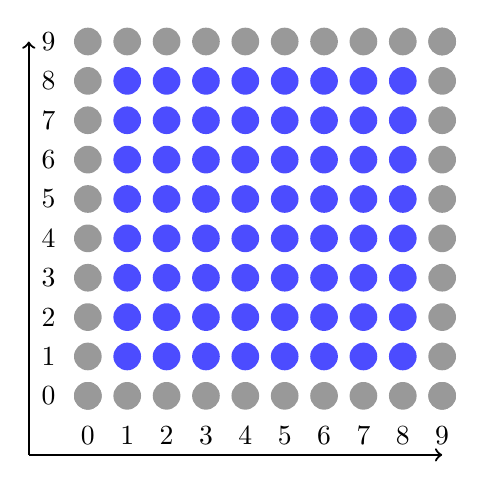
\begin{tikzpicture}[scale=0.50, auto,swap]
			%Adding the ghost nodes along the edges
			\foreach \pos/\name in 	{{(0,0)/},	{(1,0)/}, 	{(2,0)/},	{(3,0)/},
									 {(4,0)/},	{(5,0)/}, 	{(6,0)/},	{(7,0)/},
									 {(8,0)/},	{(9,0)/}}
			\node[ghost] (\name) at \pos {$\name$};
			\foreach \pos/\name in 	{			{(0,1)/}, 	{(0,2)/},		{(0,3)/},
									{(0,4)/},	{(0,5)/}, 	{(0,6)/},		{(0,7)/},
									{(0,8)/}, 	{(0,9)/}}
			\node[ghost] (\name) at \pos {$\name$};
			\foreach \pos/\name in 	{{(0,0)/},	{(1,9)/}, 	{(2,9)/},		{(3,9)/},
									 {(4,9)/},	{(5,9)/}, 	{(6,9)/},		{(7,9)/},
									 {(8,9)/}, 	{(9,9)/}}
			\node[ghost] (\name) at \pos {$\name$};
			\foreach \pos/\name in 	{{(9,0)/},	{(9,1)/}, {(9,2)/},		{(9,3)/},
									 {(9,4)/},	{(9,5)/}, {(9,6)/},		{(9,7)/},
									 {(9,8)/},	{(9,9)/}}
			\node[ghost] (\name) at \pos {$\name$};
			%Adding true grid
			\foreach \pos/\name in 	{{(1,1)/},	{(2,1)/},	{(3,1)/},	 {(4,1)/},
									{(5,1)/}, 	{(6,1)/},	{(7,1)/},	 {(8,1)/}}
			\node[true] (\name) at \pos {$\name$};
			\foreach \pos/\name in 	{{(1,2)/},	{(2,2)/},	{(3,2)/},	 {(4,2)/},
									{(5,2)/}, 	{(6,2)/},	{(7,2)/},	 {(8,2)/}}
			\node[true] (\name) at \pos {$\name$};
			\foreach \pos/\name in 	{{(1,3)/},	{(2,3)/},	{(3,3)/},	 {(4,3)/},
									{(5,3)/}, 	{(6,3)/},	{(7,3)/},	 {(8,3)/}}
			\node[true] (\name) at \pos {$\name$};
			\foreach \pos/\name in 	{{(1,4)/},	{(2,4)/},	{(3,4)/},	 {(4,4)/},
									{(5,4)/}, 	{(6,4)/},	{(7,4)/},	 {(8,4)/}}
			\node[true] (\name) at \pos {$\name$};
			\foreach \pos/\name in 	{{(1,5)/},	{(2,5)/},	{(3,5)/},	 {(4,5)/},
									{(5,5)/}, 	{(6,5)/},	{(7,5)/},	 {(8,5)/}}
			\node[true] (\name) at \pos {$\name$};
			\foreach \pos/\name in 	{{(1,6)/},	{(2,6)/},	{(3,6)/},	 {(4,6)/},
									{(5,6)/}, 	{(6,6)/},	{(7,6)/},	 {(8,6)/}}
			\node[true] (\name) at \pos {$\name$};
			\foreach \pos/\name in 	{{(1,7)/},	{(2,7)/},	{(3,7)/},	 {(4,7)/},
									{(5,7)/}, 	{(6,7)/},	{(7,7)/},	 {(8,7)/}}
			\node[true] (\name) at \pos {$\name$};

			\foreach \pos/\name in 	{{(1,8)/},	{(2,8)/},	{(3,8)/},	 {(4,8)/},
									{(5,8)/}, 	{(6,8)/},	{(7,8)/},	 {(8,8)/}}
			\node[true] (\name) at \pos {$\name$};
			%Adding numbering
			\foreach \pos/\name in 	{{(0,-1)/0},	{(1,-1)/1}, 	{(2,-1)/2},	{(3,-1)/3},
									 {(4,-1)/4},	{(5,-1)/5}, 	{(6,-1)/6},	{(7,-1)/7},
									 {(8,-1)/8},	{(9,-1)/9}}
			\node[numbering] (\name) at \pos {$\name$};
			\foreach \pos/\name in 	{{(-1,0)/0},	{(-1,1)/1}, 	{(-1,2)/2},		{(-1,3)/3},
									{(-1,4)/4},		{(-1,5)/5}, 	{(-1,6)/6},		{(-1,7)/7},
									{(-1,8)/8}, 	{(-1,9)/9}}
			\node[numbering] (\name) at \pos {$\name$};
			\draw[->, black, thick] (-1.5,-1.5) -- (9,-1.5);
			\draw[->, black, thick] (-1.5,-1.5) -- (-1.5,9);
		\end{tikzpicture}
		\caption{Dirichlet boundary conditions}
		\label{fig:dirichlet}
		\end{subfigure}
	\end{figure}
